%!TEX root = Bericht.tex
\graphicspath{{graphics/HMI/}{graphics/control_modes/}}
\chapter{The different Control Modes}
\label{cha:DifferentControlModes}

\begin{table}[H]		% [H] indicates that the table should be right here.
	\begin{tabular}{c c c c c} %{p{0.16\textwidth}p{0.16\textwidth}p{0.16\textwidth}p{0.16\textwidth}p{0.16\textwidth}}	% add p{size_of_column} for every new column you'd like to have. If you put a | between the p then there is a vertical line between the columns. 
	Test Phase 		& Direct Control 	& Assisted Control 	& Half Automatic	& Full Automatic  \\
	\toprule[1.25pt]				%define the line thickness of the top rule
	Thrust 1		& Thrust $x$	& Velocity $x$	& Velocity	& Velocity	\\
	Thrust 2		& Thrust $y$	& \textit{Velocity $y$}	& Rotation $x$	& Rotation $x$\\
	Thrust 3		& Thrust $z$	& \textit{Velocity $z$}	& Rotation $y$	& Waypoints	\\
	Thrust 4		& Moment $x$	& Rotation $x$	& Rotation $z$	&	Camera target\\
	Direction 1		& Moment $y$	& Rotation $y$	& Waypoints	&	\\
	Direction 2		& Moment $z$	& Rotation $z$	&		&	\\
	Direction 3		& 		& 		&		&	\\
	Direction 4		& 		& 		&		&	\\

	\bottomrule[1.25pt]
	\end{tabular} 
	\caption[The different control modes]{With the control modes, different inputs are given to the controller. The inputs in \textit{italic} are not available for \textit{Assisted RC  Control}.}
	\label{table:control_modes}
\end{table}

\begin{figure}[H] % [H] steht dafür, dass das Bild genau hier im Text sein soll.
	\begin{center}
		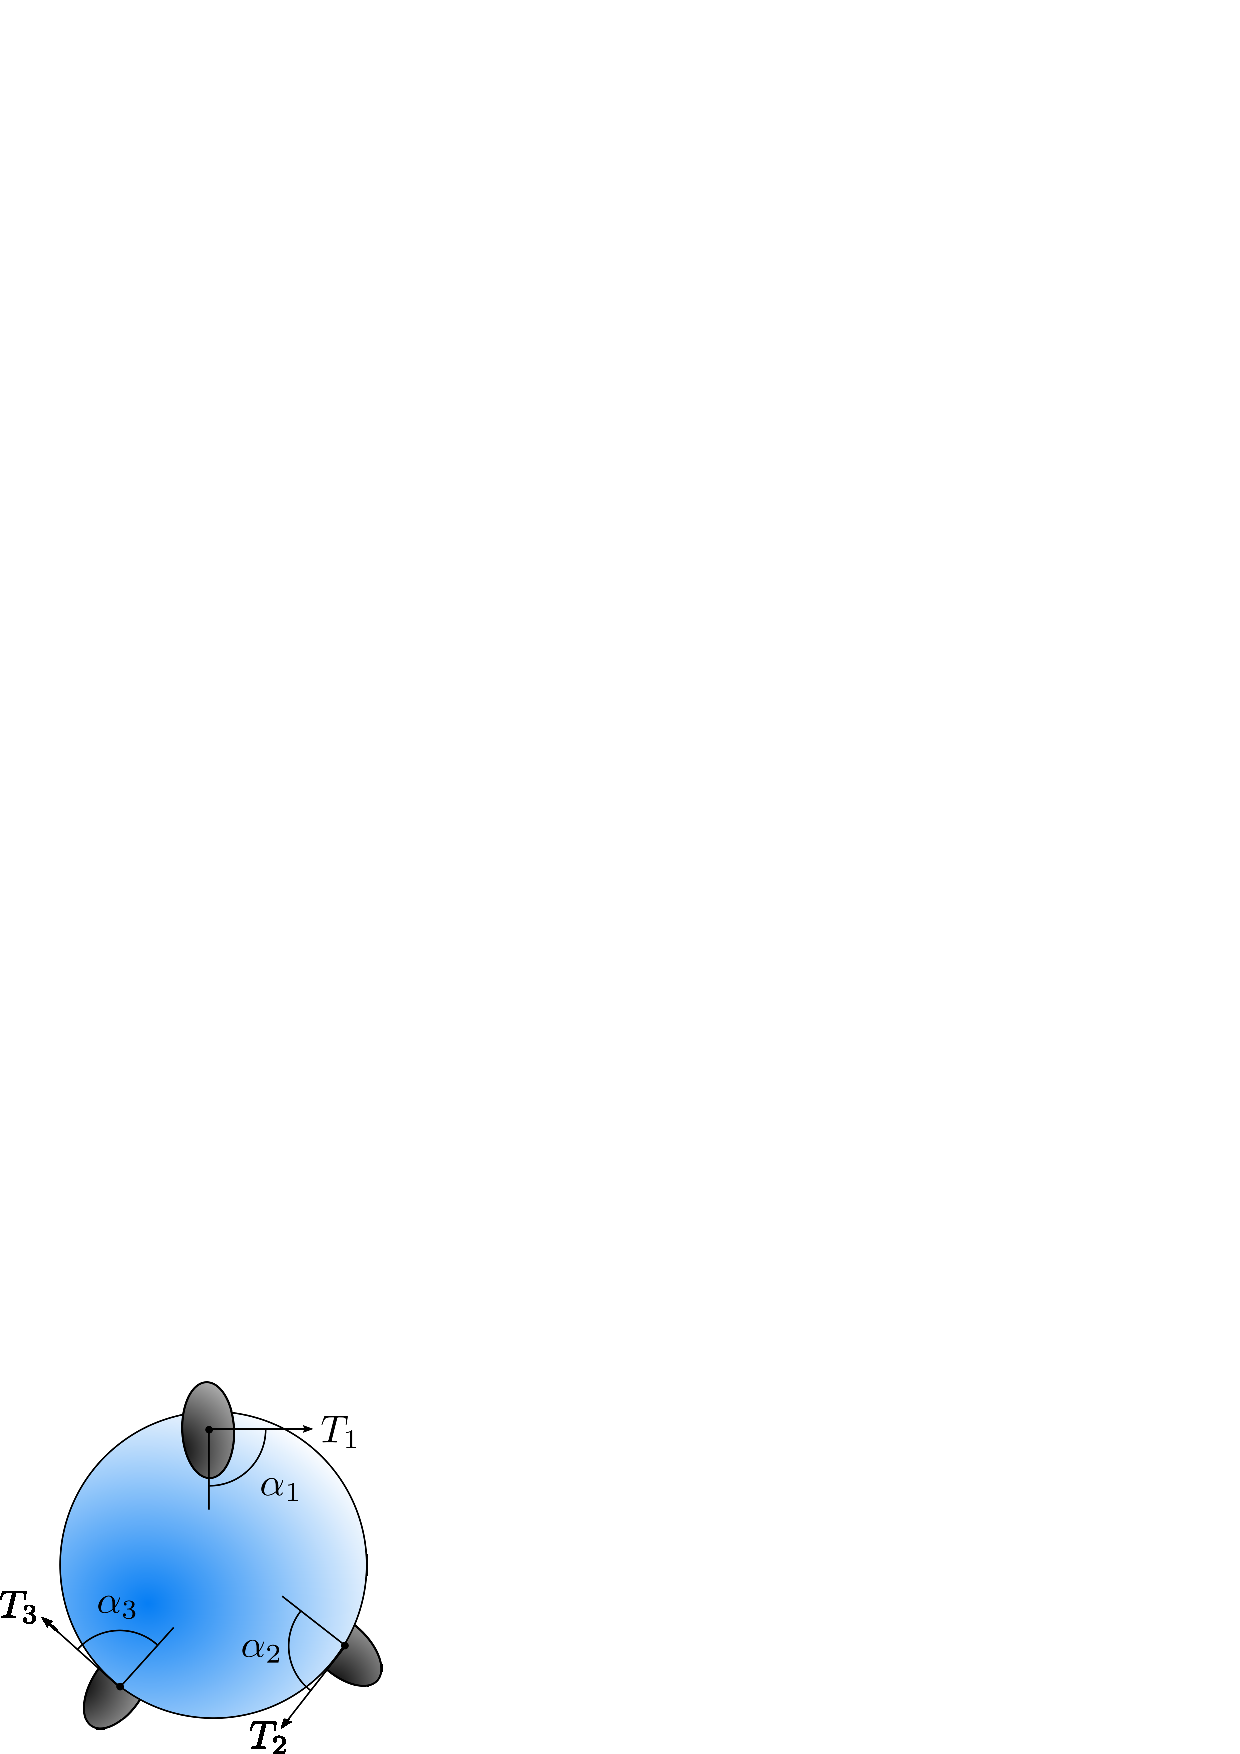
\includegraphics[width=0.3\textwidth]{TPC.pdf}
		\caption[Test Phase]{Test Phase}  
		\label{figure:test_phase}		
	\end{center}
\end{figure}

\begin{figure}[H] % [H] steht dafür, dass das Bild genau hier im Text sein soll.
	\begin{center}
		\includegraphics[width=0.3\textwidth]{DC.pdf}
		\caption[Direct control]{Direct Control}  
		\label{figure:direct_control}
	\end{center}
\end{figure}

\begin{figure}[H]		
	\small{
		\begin{center}
			\parbox{0.25\textwidth}{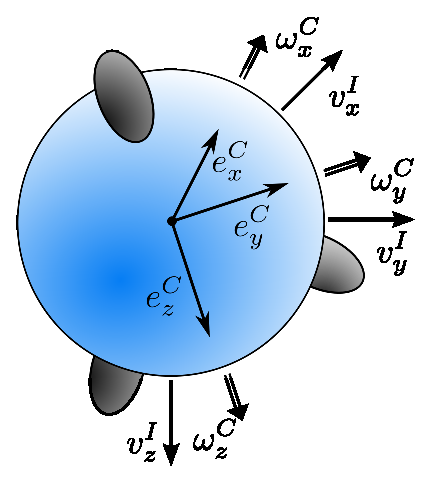
\includegraphics[width=0.25\textwidth]{AC}
			 Assisted Control}
			\hspace{0.1\textwidth}			
			\parbox{0.25\textwidth}{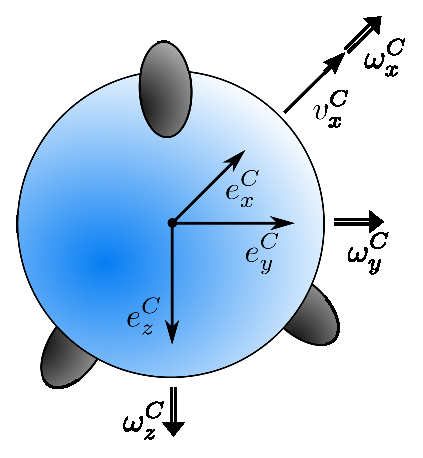
\includegraphics[width=0.25\textwidth]{RC}
			Assisted RC Control}
	\caption[Assisted Control]{Assisted Control with controlling six (left) and four (right) stabilized degrees of freedom.}
		\label{figure:assisted_control}
		\end{center}
	}			
	\vspace{4.5mm}
\end{figure}

\begin{figure}[H] % [H] steht dafür, dass das Bild genau hier im Text sein soll.
	\begin{center}
		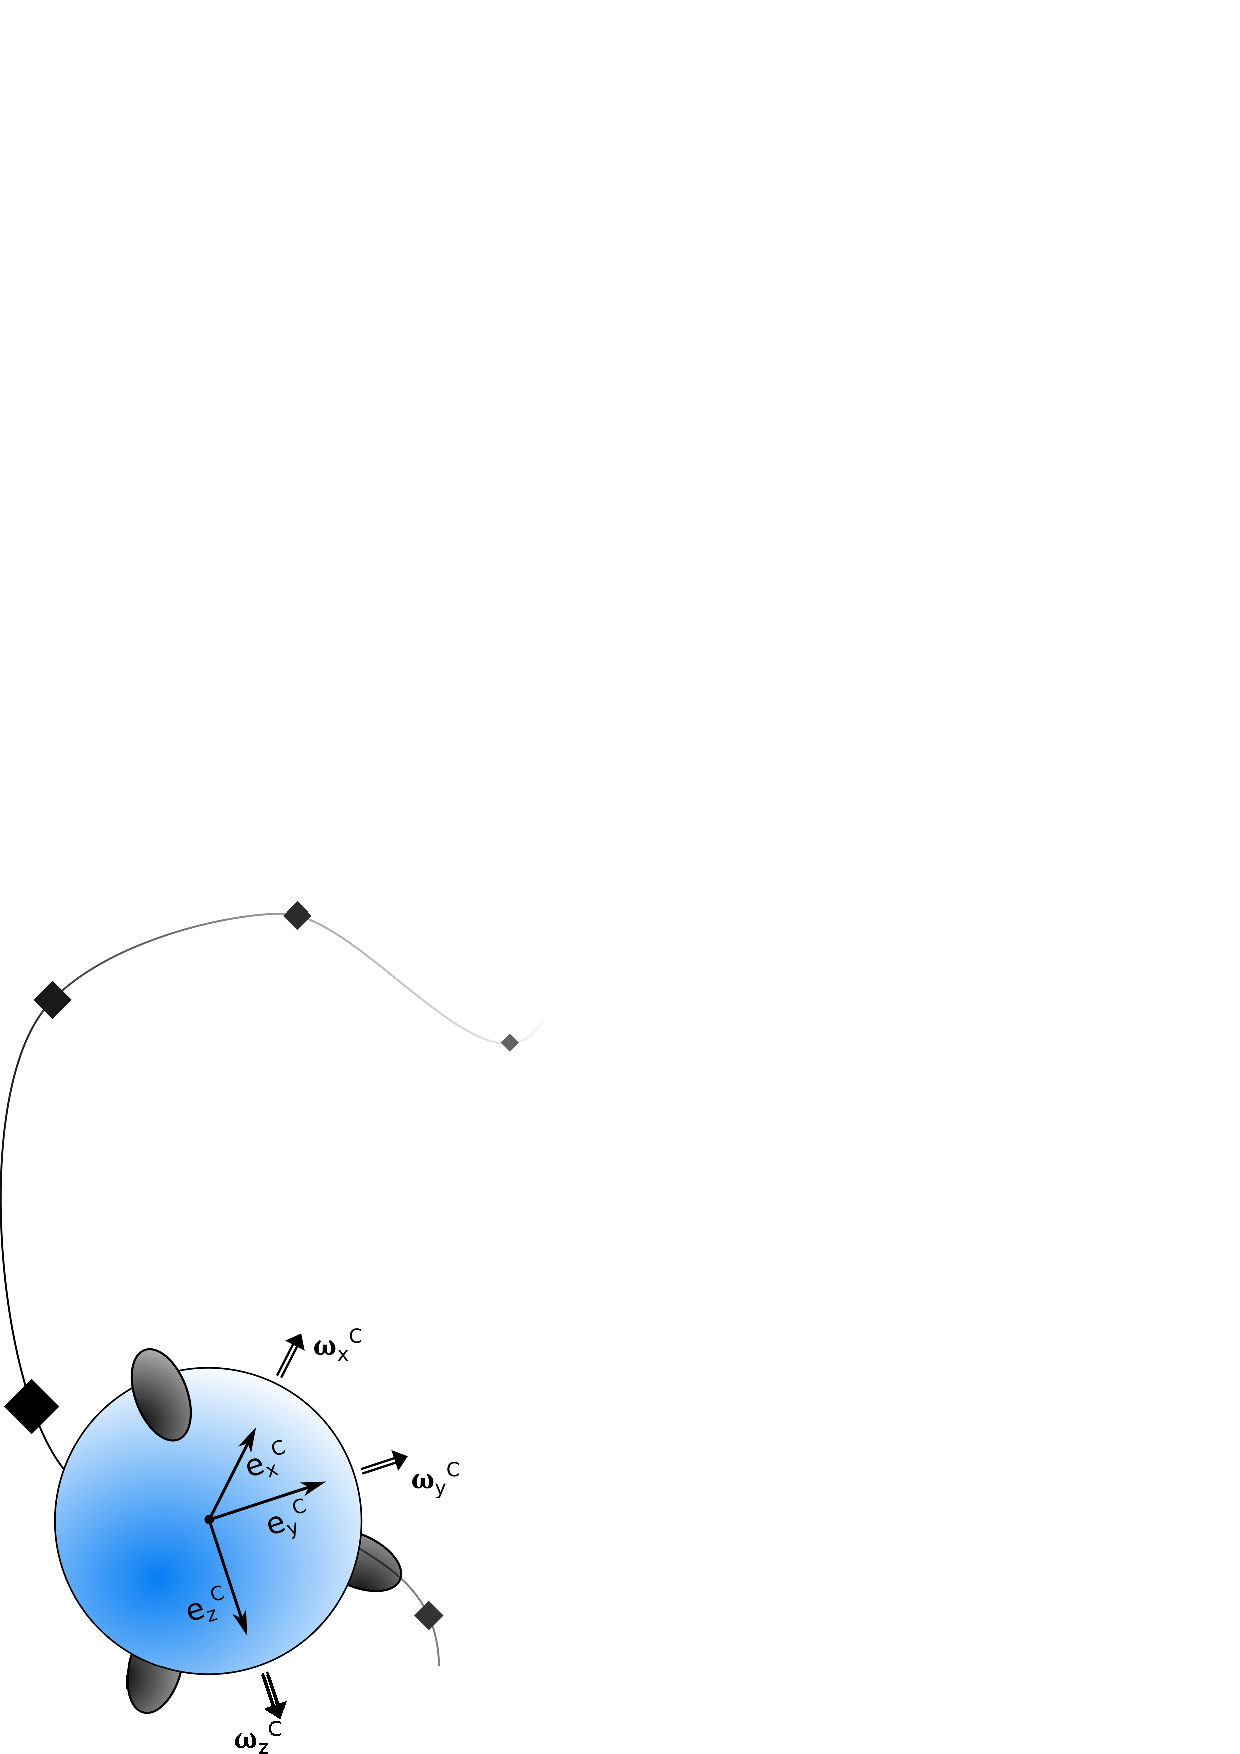
\includegraphics[width=0.4\textwidth]{HAC.pdf}
		\caption[Half automatic control]{Half Automatic Control}  
		\label{figure:half_automatic_control}		
	\end{center}
\end{figure}


\begin{figure}[H] % [H] steht dafür, dass das Bild genau hier im Text sein soll.
	\begin{center}
		\includegraphics[width=0.4\textwidth]{FAC.pdf}
		\caption[Full automatic control]{Full Automatic Control.}  
		\label{figure:full_automatic_control}		
	\end{center}
\end{figure}


\section{Elaboration}
\label{sec:elaboration}
\textit{About the need of different modes, the requirements of image capturing and overview of the realized modes}
\section{Manual Control Modes}
\label{manualControlModes}
\textit{Direct Control and Assisted Control}
\section{Automatic Control Modes}
\label{automaticControlModes}
\textit{Half Automatic Control and Full Automatic Control}